\section{eo\-Pareto\-Ranking$<$ EOT $>$ Class Template Reference}
\label{classeo_pareto_ranking}\index{eoParetoRanking@{eoParetoRanking}}
Straightforward pareto ranking.  


{\tt \#include $<$eo\-Pareto\-Ranking.h$>$}

Inheritance diagram for eo\-Pareto\-Ranking$<$ EOT $>$::\begin{figure}[H]
\begin{center}
\leavevmode
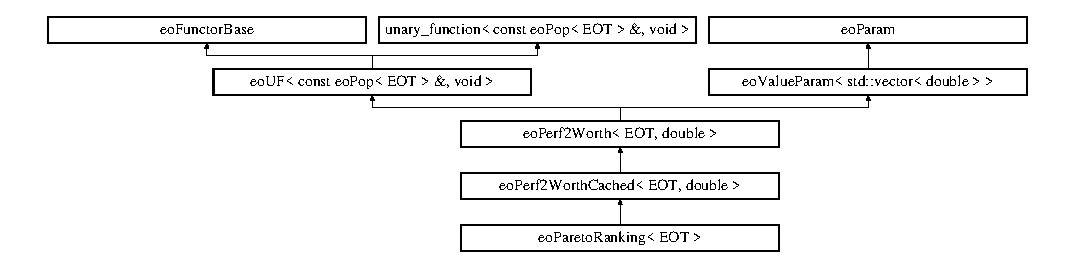
\includegraphics[height=3.15315cm]{classeo_pareto_ranking}
\end{center}
\end{figure}
\subsection*{Public Member Functions}
\begin{CompactItemize}
\item 
{\bf eo\-Pareto\-Ranking} ({\bf eo\-Dominance\-Map}$<$ {\bf EOT} $>$ \&\_\-dominance\-Map)\label{classeo_pareto_ranking_a0}

\item 
void {\bf calculate\_\-worths} (const {\bf eo\-Pop}$<$ {\bf EOT} $>$ \&\_\-pop)\label{classeo_pareto_ranking_a1}

\begin{CompactList}\small\item\em The actual virtual function the derived classes should implement. \item\end{CompactList}\end{CompactItemize}
\subsection*{Private Attributes}
\begin{CompactItemize}
\item 
{\bf eo\-Dominance\-Map}$<$ {\bf EOT} $>$ \& {\bf dominance\-Map}\label{classeo_pareto_ranking_r0}

\end{CompactItemize}


\subsection{Detailed Description}
\subsubsection*{template$<$class EOT$>$ class eo\-Pareto\-Ranking$<$ EOT $>$}

Straightforward pareto ranking. 

Every individual gets a rank according to the number of elements it dominates. Note that without niching, this technique will usually not find the whole front of non-dominated solutions, but will quite likely converge on a single spot on the front. 



Definition at line 40 of file eo\-Pareto\-Ranking.h.

The documentation for this class was generated from the following file:\begin{CompactItemize}
\item 
eo\-Pareto\-Ranking.h\end{CompactItemize}
